\subsection*{Overview of an Existing System}
% - Describe the existing system from which you are to improve for your
%  proposed research project.  Include its system architectures where
%  appropriate
% - Stress a specific area of the existing system where you are to focus on and
%  indicate the value of your research and its contribution to the field.
The game that we have drawn inspiration from is a 1980’s arcade game
known as Galaga. Galaga was developed by Namco in 1981 and is a
shooter based game where the player tries to take down enemy ships
by shooting at them. The enemy ships may be taken down in one or two
hits. Enemy ships requiring two hits are known as the Galaga and
will turn blue after the first hit, indicating that there is one hit
left to take down the ship. While shooting at enemy ships the player
must also avoid being hit by enemy fire while also avoiding the beam
from the Galaga looking to capture a players’ ship. If captured the
players ship will remain imprisoned unless the Galaga is taken down.

Galaga's gameplay consists of managing the movement and firing of a
ship in order to avoid incoming projectiles whilst scoring hits on
enemy ships by firing their own. The crux of this system's
architecture as well as our own is the ship class. The fields for
the ship class include both a \mintinline{python}{rect} used for
determining the position of the ship and an image to represent it.
In addition to a method for movement, a method for firing exists,
which creates a projectile object. The projectile class possesses the
same fields as the ship, but lacks the method for firing.

A significant portion of the user's attention is drawn to the paths
of moving projectiles. Our improvement upon this system is to do
away with the projectile in favor of adding a weapon class which
possesses a method to instantaneously draw a laser beam on the
screen and register damage to the enemies hit by it. This instant
damage allows the user to hit fast-moving targets by virtue of
reaction time rather than by prediction projectile and ship
movements. To introduce extra challenge for the user, both the ship
and weapon class have color as a property. When registering damage,
a weapon only damages a ship of matching color. A ship possesses a
list of weapons and a method to switch the active weapon and fire
it. This addition creates an imperative to match their ship's active
weapon to the color of the enemy they are firing upon.

An open-source clone of Galaga which we chose to examine and improve
upon is \href{https://code.google.com/archive/p/pylaga/source/default/source}{Pylaga}.
Pylaga is an implementation of Galaga written in python, and using
pygame.  It is, therefore, an easy system to compare to our own.
Pylaga's enemies and players lack our concept of color.  Pylaga's
class structure is as follows:

\begin{figure*}
    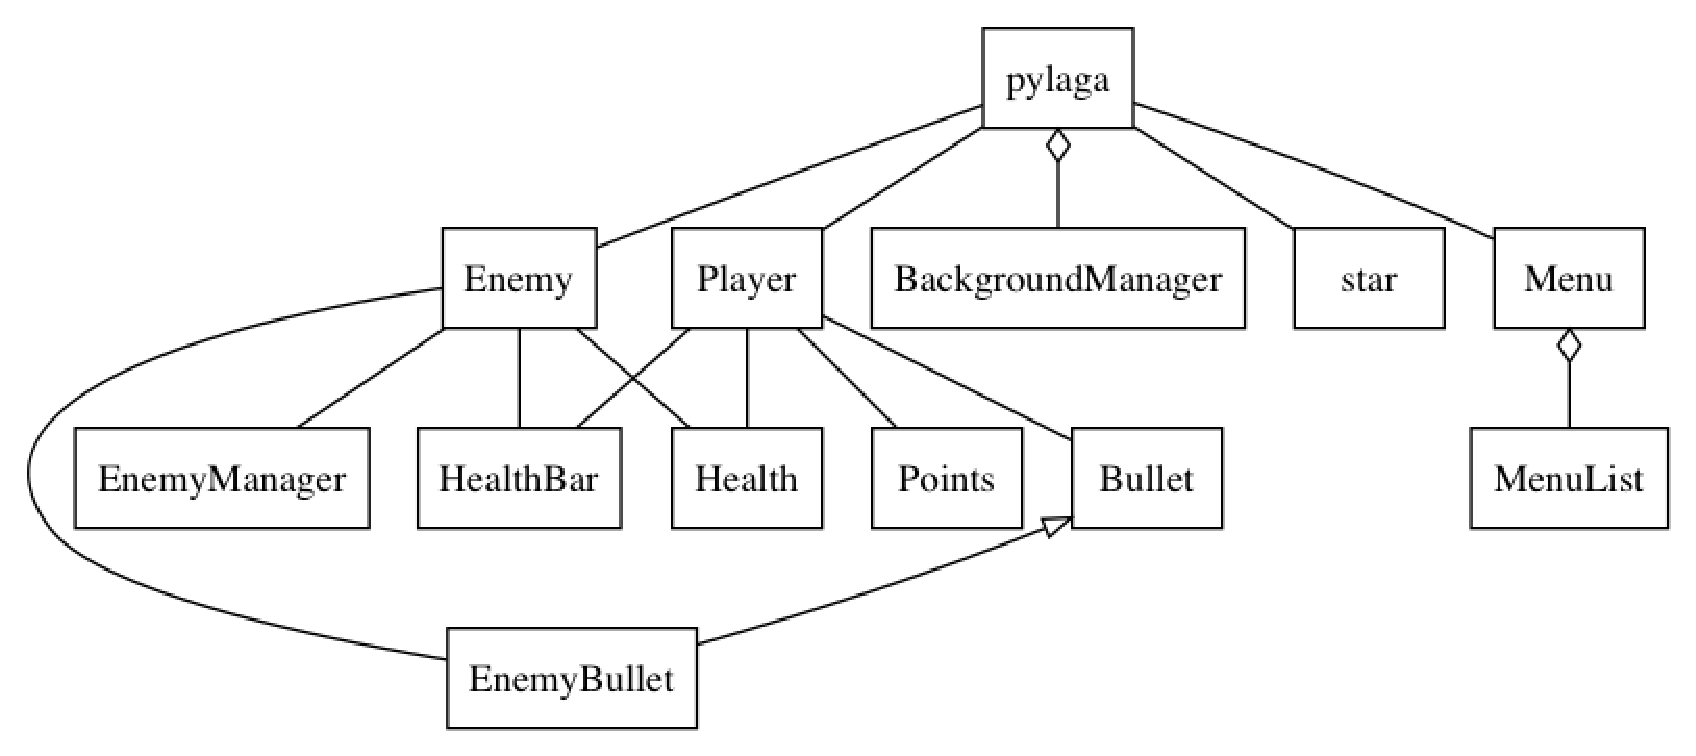
\includegraphics[width=0.75\textwidth]{../images/pylaga}
    \caption{Pylaga's Class Diagram}
\end{figure*}

It is clear from the above diagram that the author did not implement
class inheritance, but used classes just for identification purposes
and for storing some functionality.  Much of the actual data was not
encapsulated, but stored in global variables.  Our version will be a
marked improvement upon this. In particular, objects on the screen
will inherit from the \mintinline{python}{RenderedBase} class, and
moving objects will inherit the relevant code from
\mintinline{python}{ActorBase}.  This will lead to greater maintainability
and core re-use.

\begin{figure*}
    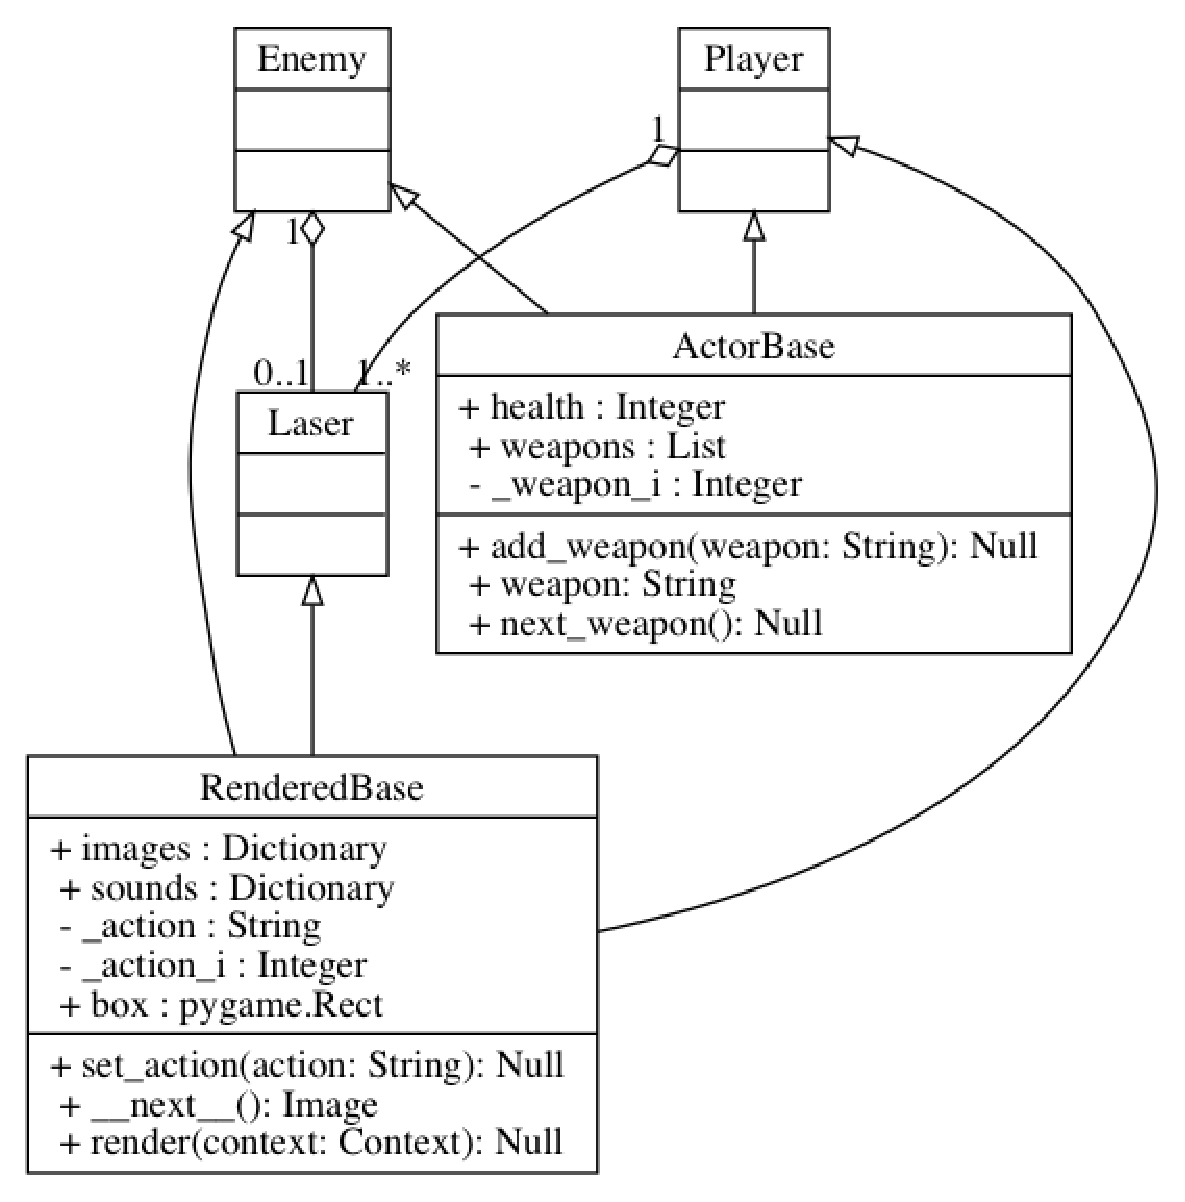
\includegraphics[width=0.75\textwidth]{../images/object_models}
    \caption{Our Class Diagram}
\end{figure*}

The author of Pylaga implemented a player shooting using the following
method:

\inputminted[baselinestretch=1]{python}{../code/pylaga_player.py}

This is a rather messy method, as it alters the state of its parameters,
rather than updating a member of the class.  Our proposed algorithm,
below, will be a substantial improvement upon it.

For rendering images, the author of Pylaga chose to use global variables
which are accessed and updated in each class's \mintinline{python}{update}
method.  The definitions and the update methods are:

\inputminted[baselinestretch=1]{python}{../code/pylaga_images_and_update.py}

The use of global variables here exhibits low cohesion among the
components of the game.  No other components but the player class
are concerned with what image the player is represented with; yet
all have access.  Our system will leverage python's \mintinline{python}{__next__}
``magic method'' (also known as a ``dunders'' method) to increase component
cohesion.

\subsection*{The Proposed System}
Our proposed system is ``Lazer Blast'', an arcade-style shooter (like
\href{https://en.wikipedia.org/wiki/Galaga}{Galaga}), which includes
aspects of color matching and pattern matching similar to Simon.

\subsubsection*{Game-play}
The user pilots a small ship against hoards of enemies.  Each enemy
has a given color.  The player must use a similar-colored laser to
destroy that enemy.  For example, an enemy which is green much be
shot with a green laser.  A red laser will have no effect on a green enemy.
Waves of enemies come in patterns: an astute fighter will be able to
predict the next wave from the previous, and will have a significant
advantage over the enemy.

Since the player cannot be expected to handle the copious masses
of colorful enemies immediately, the difficulty of the game increases
as the player progresses, starting with a single color and slowly
adding other colors and increasing the speed.

\subsubsection*{System Architecture}
Lazer Blast was designed using Object-Oriented Design, and implemented
with an Object-Oriented Approach using Python and the game library,
\href{http://pygame.org/news}{pygame}.  Python was choosen for the
ability to rapidly prototype, as well as its widespread use among
the open-source community.  Object-Oriented Programming is well
adapted to Python: Python, while being a multi-paradigm language,
has a strong tendency towards Object-Oriented Programming.  The
framework, pygame, was chosen due to its relative simplicity and due
to its relative impartiallity towards individual implementation choices.

In the Object-Oriented Design, all objects which are drawn to the screen
are subclasses of the \mintinline{python}{RenderedBase} class.  All
objects which perform some action subclass the \mintinline{python}{ActorBase}
class.  For example, obstacles will be subclasses of
\mintinline{python}{RenderedBase}, but all enemies will be subclasses of
\mintinline{python}{ActorBase} and of \mintinline{python}{RenderedBase}.
For the initial version of the game, there is only one obstacle,
\mintinline{python}{Obstacle}, and only two types of actors:
\mintinline{python}{Player} and \mintinline{python}{Enemy}.

% Class diagram of RenderedBase, ActorBase, Obstacle, Enemy, and Player.

In addition to the \mintinline{python}{RenderedBase} and
\mintinline{python}{ActorBase} classes, there is also the
\mintinline{python}{Menus} class. The few menu screens that there are
will be subclasses of \mintinline{python}{Menus} and include the Main
Menu, High Scores, and Options screens, which can each be built off of
the \mintinline{python}{Menus} class by simply changing the graphics
on that screen.

\subsubsection*{Algorithms}

% Algorithms
Gratuitous use of Python's magic method, \mintinline{python}{__next__}
was made to implement all sequential algorithms that were necessary.
In this way, each object which maintained a state through a sequence
acts as a generator.  This eases the complexity of logic, and makes
maintaining state easier. (As the individual components exhibit looser
coupling, and stronger cohesion.)  For example, the images to be blitted
to the screen for a given actor are defined as follows:

\inputminted[baselinestretch=1]{python}{../code/RenderedBase.py}

The \mintinline{python}{GameSound} class will implement the sound
aspects of the game.  It will provide the lasers with sound every
time they are activated, will play a crashing sound when a specific
colored laser hits the matching colored target and will provide a
sound specific to the player losing or winning the game.

\inputminted[baselinestretch=1]{python}{../code/GameSound.py}

Our primary improvement over Galaga and Galaga-like clones is
adding a color component.  The actual logic for this component
is simple.  The \mintinline{python}{LaserStrike} class will display a
laser object of a specific color when a certain key is selected. If
the laser is of the same color as the enemy target and makes contact,
then this class will call the \mintinline{python}{GameSound} class
in order to implement the crashing sound that will return from a
direct hit. This class will also call the \mintinline{python}{Enemy}
class in order to deduct health upon a hit.

\inputminted[baselinestretch=1]{python}{../code/LaserStrike.py}

As for algorithms that may be used in \mintinline{python}{Menus}, they
are fairly straightforward. For the most part, the only input that a
user can make on a menu is moving the cursor, and that is simply
incrementing and decrementing a counter based on which direction the
user inputs, and this counter is read in order to redraw the cursor on
the screen so that the user can see which selection they have highlighted.
The only other input a user can make is selection, which moves the user
from the current menu to another screen, or closes the application. The
current menu is assigned by a variable to know which graphic to render for
the user.
